\section{Data Management Framework (DMF)}
\label{sec.dmf}
The Data Management Framework (DMF) provides a central,
network-accessible service to archive and track all files related to a
carbon capture investigation. It facilitates group interactions by
providing a venue to share documents between multiple, geographically
distributed individuals while tracking the relationships between these
files. It is intended to store all the data related to a project from
the gathering of experimental data, to the development of basic
models, to the development of process models, and ultimately
optimization and UQ studies.

In addition to providing basic file sharing services, the DMF is setup
to store multiple revisions of each file in the system and it
provides a historical archive of the evolution of the project. Older
version of data and model files are stored to enable backtracking or
to provide a means to compare the final product with earlier work.

The DMF can also be used to track the provenance of simulation
results. As files are added to the DMF, the user specifies
relationships between individual files to indicate a dependency. For
example, a basic model file depends on a file containing experimental
data, and a process model file depends on the basic model
file. Collections of these dependency relationships help establish
the provenance chain for each file in the system. This enables DMF
users to see when dependencies of a simulation
have been modified, indicating that the simulation may not be
incorporating the best available data.

A lightweight version of the DMF (known as the DMF lite), is also now available.
The DMF lite provides fewer functionalities than its server-based counterpart.
Version control and metadata for data objects are provided in the DMF lite,
but provides no search and minimal dependency tracking functionality (only tracks
dependencies for simulations). It is designed to work locally without the
need for a centralized server.

This section discusses the various components bundled with FOQUS.
There are three main components, which enables the user to open,
save, browse, and edit files in the DMF. A separate tool for
ingesting basic data models is also bundled in FOQUS. These are discussed in
more detail in the subsections below.

\subsection{Setup for Use with FOQUS}
\label{dmf-setup}

The DMF has two modes. It can be setup to be used on the local machine (DMF lite) or with a server.
The former, DMF lite, depends on Git as its backend while the latter uses an Alfresco data repository as its backend.
Both modes can be operated independently of each other. Setup instructions for both modes are specified below.

\subsubsection{DMF Lite}
The DMF is a lightweight DMF that requires minimal dependencies and is meant to be used by a single user.
In the case of the DMF lite, the Git distributed version control system is all that needs to be installed.
The DMF lite
was developed with Git version 2.5.0, but should work with newer versions as well. When
installing Git on Windows, the options (1) Use Git from the Windows Command Prompt and
(2) Checkout as-is, commit Unix-style line endings should be selected.

Certain features in the DMF lite are meant to be synced with a server. If these features are desired,
instructions in the following subsection will be needed.

\subsubsection{DMF (with Server)}
\label{dmf-with-server}
To enable FOQUS to access the server-based DMF, the following steps are needed:
\begin{enumerate}
\item Creation of properties file.
\item Execution of build script.
\item Installation of certificates (Note: This is only needed if server uses the https protocol.)
\end{enumerate}
Each step is independent and does not need to be executed in order. More details are provided below.

\textbf{Properties file:}
For each server-based DMF, a
.properties file (files that have .properties as an extension) must first be created. Multiple
.properties files can be added to enable access to multiple servers.
These files provide the configuration information that
is needed for FOQUS to locate one or more DMF repositories.
(\textbf{Important:} It is important that the file ends with the .properties extension. The fields
specified in the .properties file are also case-sensitive.)

For Windows systems, these files must be placed under the ``\%APPDATA\%'' directory.
For Linux or OS X systems, the files must be placed under the ``\$HOME'' directory.

The .properties file must consist of the following fields:

alfresco\_atompub\_url=/alfresco/cmisatom\\
auth\_http\_basic=true\\
cookies=true\\
IP\_ADDRESS=dmf-test-vm.lbl.gov\\
PORT=443\\
PROTOCOL=http://\\
repo\_name=My Test Repo\\

The IP\_ADDRESS variable should
point to the location of the DMF server and the PORT variable, the port number on which
the server was setup. ``repo\_name'' is used for specifying a name that describes the
current DMF repository.

Use of the DMF components requires Java (1.8 or later) and the JAVA\_HOME variable being defined.
FOQUS allows setting the ``JAVA\_HOME'' variable in the \textbf{\underline{Settings}} button drop-down menu.
For the DMF browser component, this will need to be specified within the system.

\textbf{Build script:} In addition, the ant build script (``build.xml'') needs to be executed before using the DMF by typing ``ant opencmis'' (without quotes).
This requires the installation of Apache Ant (1.9.6 or later) and the Java JDK (1.8).
The build script is located
at ``dmf\_lib/java/build.xml'' in the FOQUS bundle. Execution of the build script will download and install the
Apache Chemistry library and Alfresco OpenCMIS extension library.
Both libraries are licensed under the Apache 2.0 license.
If there are questions or errors pertaining to the use of Ant or Java, please contact the CCSI support team.

\textbf{Certificate installation:} If the DMF is used with the https (not http) protocol,
installation of certificates in the corresponding java package are
required. Instructions for certificate installation are as follows:

\begin{enumerate}
\item On the command line, find the directory ``dmf\_lib/java/cert'' in the FOQUS bundle.
\item Run the command: ``\$JAVA\_HOME/bin/java InstallCert''. On Windows the command will be ``\%JAVA\_HOME\%\textbackslash bin\textbackslash java InstallCert''.
The command takes in a hostname and a secure port number, the default https port will be 8443 (for example, ``localhost:8443''). An optional passphrase can also be passed in.
\item If prompted, select the default option and a certificate with the name of ``jssecacerts'' will be generated.
\item Copy the certificate to ``\%JAVA\_HOME\%\textbackslash jre\textbackslash lib\textbackslash security\textbackslash'' for Windows. On Mac/Linux platforms, copy the certificate to
``\$JAVA\_HOME/jre/lib/security''.
\end{enumerate}

After configuring the property files and environment variables, there is one last step required to allow FOQUS to use the DMF.
Under the FOQUS \textbf{\underline{Settings}} button, \textbf{\underline{FOQUS}} tab, select the \textbf{\underline{Use DMF if available}} checkbox (Figure~\ref{fig:foqus-dmf-settings}).

\begin{figure}[H]
  \centering
  \includegraphics[width=.75\textwidth]{Chapt_flowsheet/figs/FOQUS-settings}
  \caption{Enabling the Use of DMF through FOQUS Settings Menu}
  \label{fig:foqus-dmf-settings}
\end{figure}

\begin{figure}[H]
  \centering
  \includegraphics[width=.75\textwidth]{Chapt_flowsheet/figs/DMFFoqus}
  \caption{DMF-Related Submenus in FOQUS Session Menu}
  \label{fig:foqus-dmf-menu}
\end{figure}


If the property files and environment variables are setup correctly, menu items will display with
DMF-related submenus under the FOQUS \textbf{\underline{Session}} button (Figure~\ref{fig:foqus-dmf-menu}).
The subsequent subsections assume the correct setup of these property files and environment variables.

\subsection{Login Dialog (DMF with server)}
\label{login-dialog}

\begin{figure}[H]
  \centering
  \includegraphics[width=.5\textwidth]{Chapt_flowsheet/figs/login}
  \caption{DMF Login Prompt}
  \label{fig:login-dialog}
\end{figure}

This subsection is only relevant if using the DMF with a server. If the user is
planning to use only the DMF lite, skip this subsection.
When first connecting the DMF with a server, the user is prompted with a login dialog (Figure~\ref{fig:login-dialog}).
The user should login using the username and password given by the DMF server administrator
(instructions for creating these login credentials is provided at the DMF server side).

The user has the option of saving their user credentials so that they do not have to input their login credentials every time. To delete the saved
credentials, select {\textbf{\underline{Logout from DMF Repositories}} from the
\bu{Session} button drop-down menu, mentioned in Section~\ref{session-menu} (this option will display only when the DMF is enabled).
Logging out will remove all saved credentials from all repositories.

The login dialog feature is only relevant to the DMF lite when using the upload to server feature.

\subsection{Open Dialog}
\label{open-dialog}

The DMF open dialog (Figure~\ref{fig:open-dialog}) is accessible by selecting
\bu{Open Session} in the \bu{Session} button drop-down menu (Figure~\ref{fig:foqus-dmf-menu}),
mentioned in Section~\ref{session-menu}. This dialog enables the user to select and load a session file.
Associated simulation files are also opened with the intended session file.

\begin{figure}[H]
  \centering
  \includegraphics[width=.95\textwidth]{Chapt_flowsheet/figs/open-anno}
  \caption{DMF Open Dialog Box}
  \label{fig:open-dialog}
\end{figure}

\begin{enumerate}
\item \bu{Search Repository} for files. (This feature is not present in the DMF lite mode.)
  This text bar enables the user to search the repository. Some example queries are:
  \begin {enumerate}[label=(\alph*)]
  \item Search for items created on a specific date: created:``2014-09-22''
  \item Search for items modified between a date range: modified:``2014-09-22''..``2014-10-1''
  \item Search for items created by a certain username: creator:``ccsi''
  \item Search for items with a specific title: title:``session file''
  \item Wildcards can also be used. The following example is used to find all items with words starting with ``BFB*''.
  \item Conjunctions such as \textit{and} and \textit{or} can be used to chain queries
  \end {enumerate}

\item \bu{File Browser Pane} enables the user to navigate the DMF filesystem.
  Each user can view two root folders: (1) \textbf{\underline{Shared}} and (2) \textbf{\underline{User Homes}}. By default, each user can only view their home directory
  unless permissions are given to access additional directories at the DMF server side.
  When the search repository feature is used, the file browser displays matching files or folders of the query.
  (Note: By default, the pane is hidden but can be revealed by dragging the
  splitter at the right of the dialog box.)
\item \bu{Detailed Information Pane} provides detailed file metadata. By default, this is hidden. The pane can be opened by dragging the splitter at the right.
\item \bu{Selected File Name} displays the name of the selected file in the File Browser Pane.
\item \bu{File Display Filter} enables the user to filter based on the file types. The current implementation enables filtering of JSON files rather than viewing all files types.
\end{enumerate}

\subsection{Save Dialog}
\label{save-dialog}

\begin{figure}[H]
  \centering
  \includegraphics[width=.95\textwidth]{Chapt_flowsheet/figs/save}
  \caption{DMF Save Dialog Box}
  \label{fig:save-dialog}
\end{figure}

The DMF save dialog (Figure~\ref{fig:save-dialog}) is similar to the open dialog and is accessible by selecting \bu{Save Session} in the \bu{Session} button drop-down menu
(Figure~\ref{fig:foqus-dmf-menu}, also discussed in Section~\ref{session-menu}). When a session is saved, associated simulation files are also ingested into the DMF.
The major differences between the ``open dialog'' and the ``save dialog'' are the \bu{Open} versus \bu{Save} buttons and the presence of a \bu{New Folder} button.

When \bu{New Folder} is clicked, the new folder dialog box (Figure~\ref{fig:new-folder}) displays.
There are three fields that require user input as follows:
\begin{enumerate}
\item \bu{Name} is the name of the folder and is a mandatory field, as indicated by the asterisk.
\item \bu{Description} is an optional field that enables the user to input the description of the new folder.
\item \bu{Fixed Form} accepts a true or false value: true indicates that the contents of the
folder cannot be altered; false indicates that the contents can be changed. The default for this
attribute is false (i.e., the contents can be changed).
\end{enumerate}

Similarly, when \bu{Save} is clicked, a dialog box (Figure~\ref{fig:new-file}) prompts the user to enter the session file metadata.
The following fields are associated with DMF files:
\begin{enumerate}
\item \bu{Display Name} is the name of the file and is the primary name stored in the DMF.
  This is a mandatory field as indicated by the asterisk.
\item \bu{Original File Name} is an optional field that can be used to indicate the original file name if different
  from what is saved in the DMF.
\item \bu{Description} is an optional field and enables the user to enter the description of the new file.
\item \bu{Mimetype} is a mandatory field for identifying the application that is meant to open this file.
\item \bu{External URL} is entered to specify the location of a file if stored at a remote location.
\item \bu{Version Requirements} is used to specify the version requirements of applications that use this file.
\item \bu{Confidence} specifies the stage of whether a file is experimental, at the testing stage, or the production stage. This defaults to experimental.
\end{enumerate}

\begin{figure}[H]
	\centering
	\centering
	\subfloat[New Folder dialog]{{\includegraphics[width=.25\linewidth]{Chapt_flowsheet/figs/folder-metadata}
			\label{fig:new-folder}}}%
	\qquad
	\subfloat[Save File Dialog]{{\includegraphics[width=.35\linewidth]{Chapt_flowsheet/figs/file-metadata}
			\label{fig:new-file}}}%
	\caption{Folder and File Metadata Input Dialog Box}
\end{figure}

\subsection{Browser}
The DMF Browser (Figure~\ref{fig:browser}) is a standalone tool that is bundled with the FOQUS toolsuite.
Although the browser shares the layout with the dialog boxes, there are a number of additional features.
It is meant to enable quick access to the data in the repository and view dependencies among files.
Instructions pertaining to property files and environment variables mentioned in Section~\ref{dmf-setup} are
also relevant to the use of the DMF Browser. The lite version of the DMF Browser (Figure~\ref{fig:lite-browser})
has a slightly different toolbar and
does not provide the functionality for dependency tracking.

\begin{figure}[H]
  \centering
  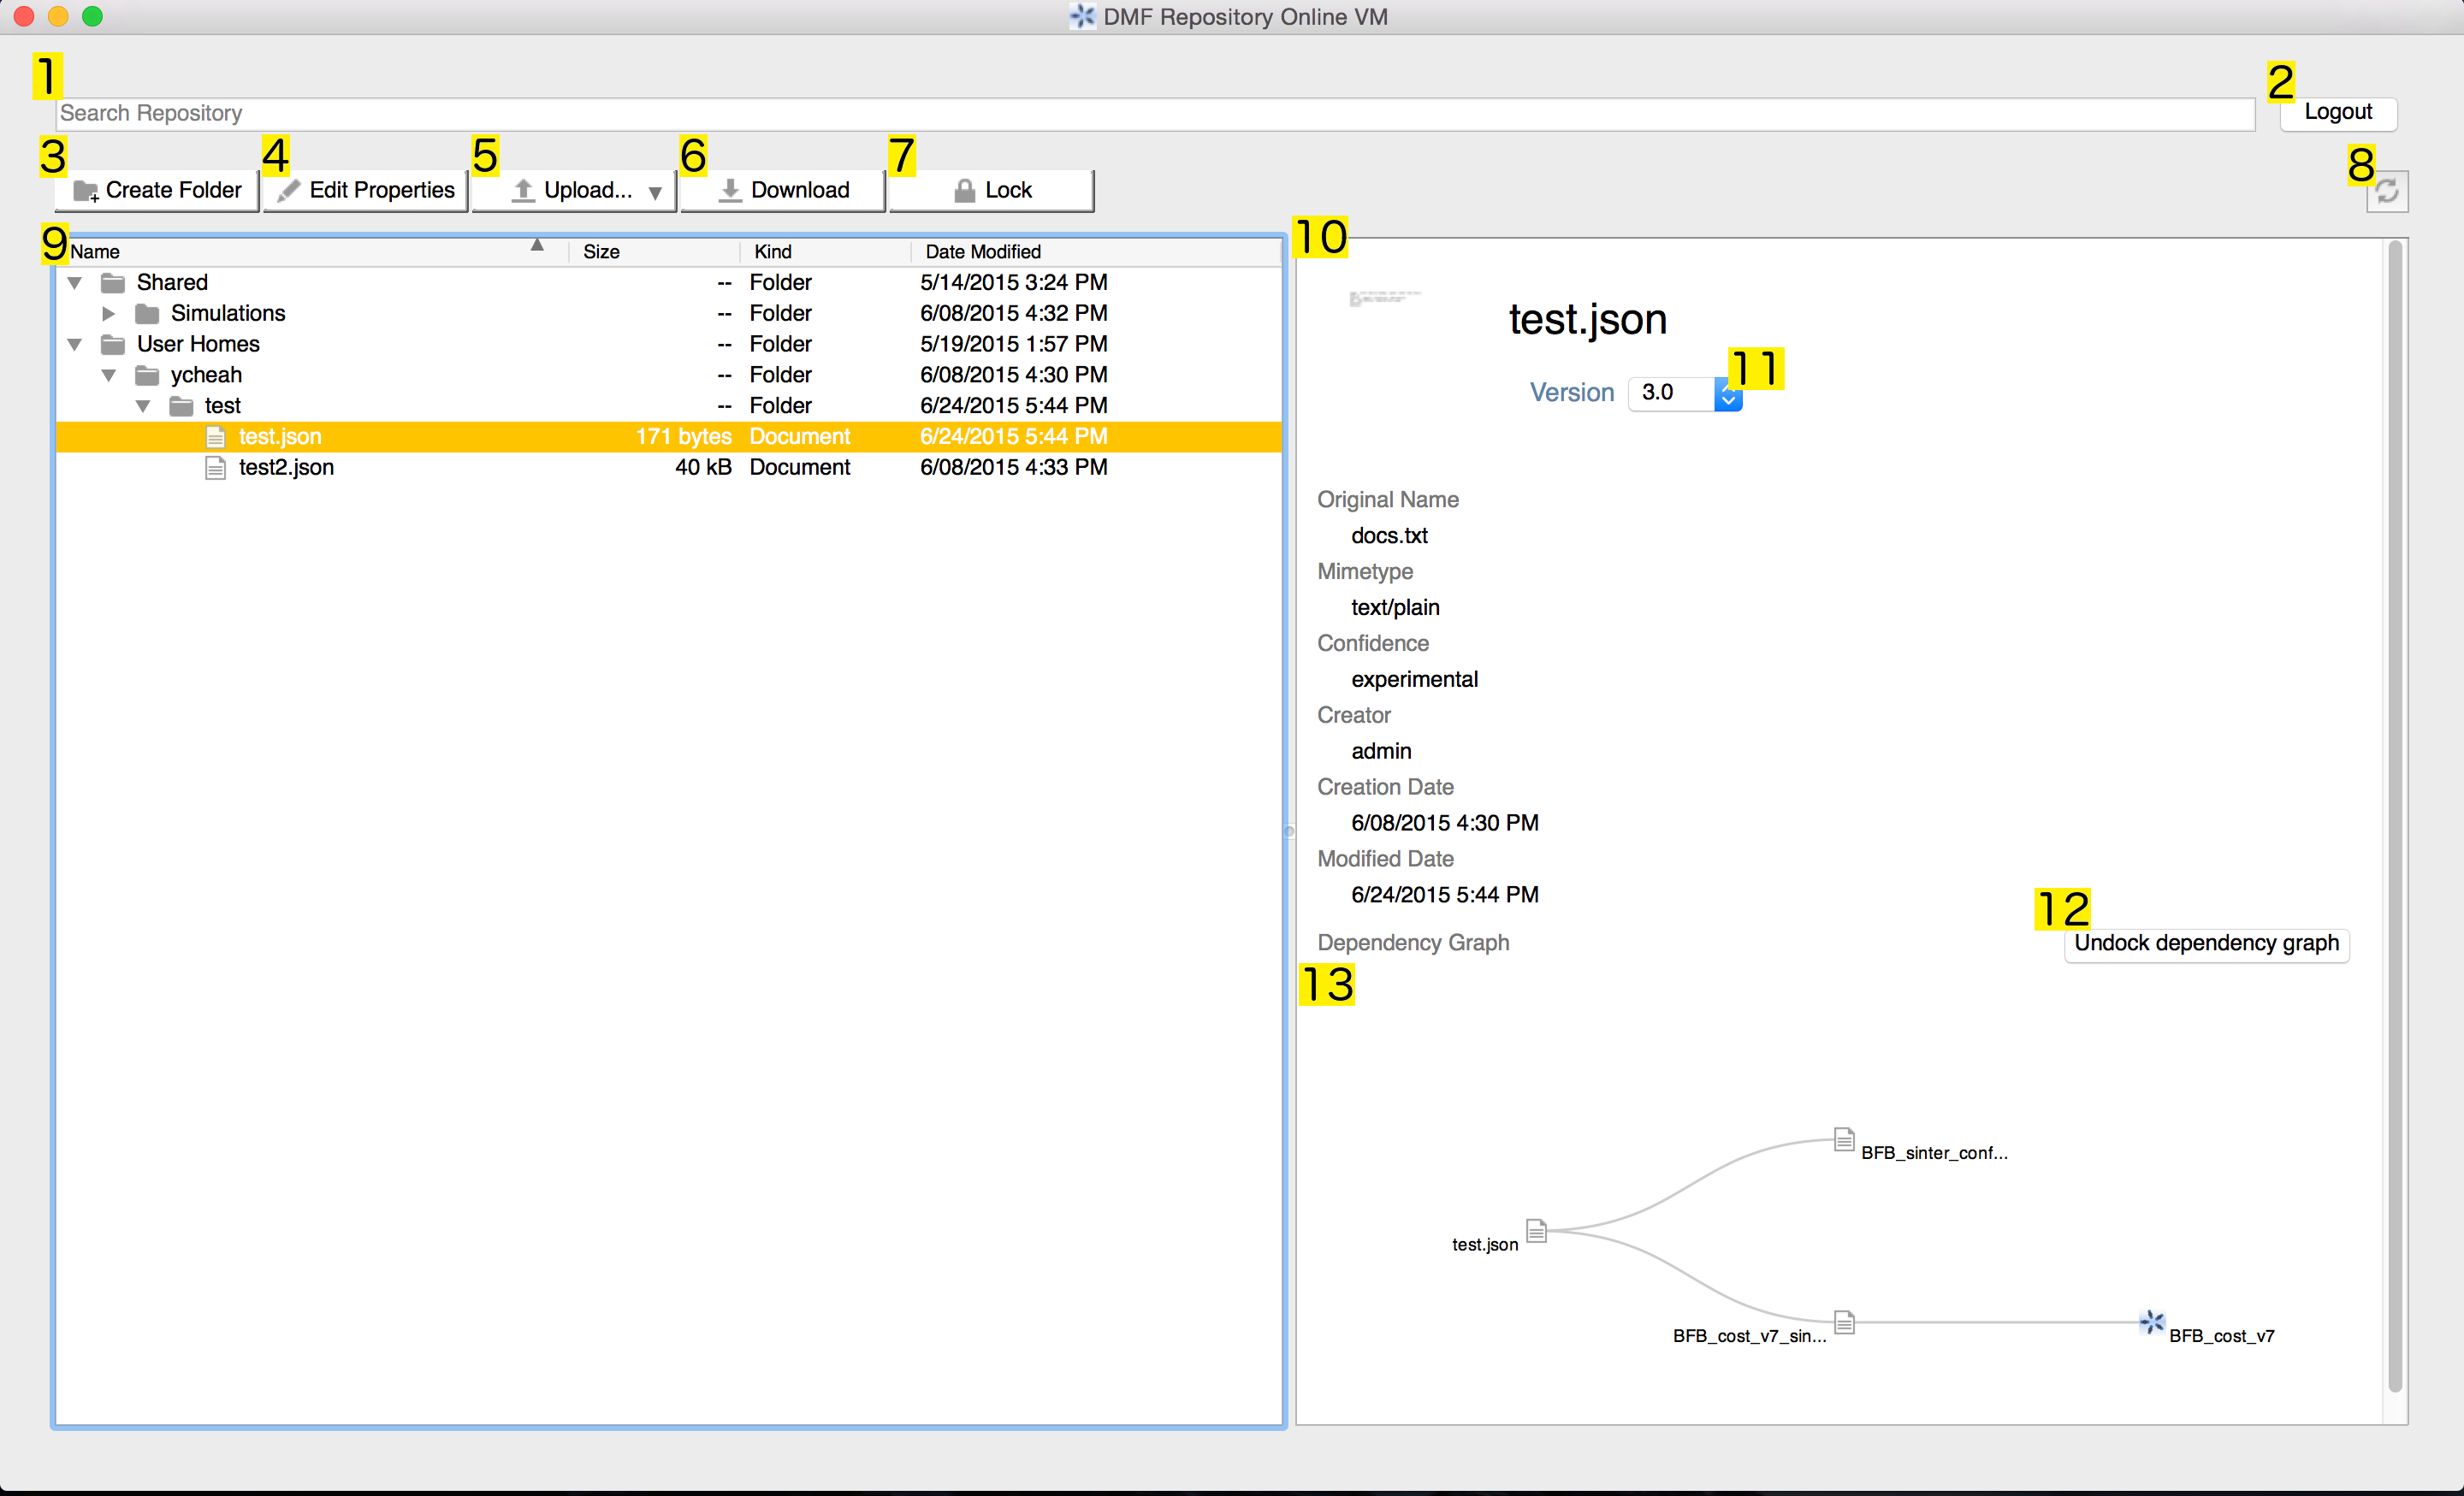
\includegraphics[width=.95\textwidth]{Chapt_flowsheet/figs/DMFBrowser}
  \caption{DMF Browser}
  \label{fig:browser}
\end{figure}

\begin{figure}[H]
  \centering
  \includegraphics[width=.95\textwidth]{Chapt_flowsheet/figs/DMFLiteBrowser}
  \caption{DMF Browser Lite Toolbar}
  \label{fig:lite-browser}
\end{figure}

\begin{enumerate}
\item \bu{Search Repository} for files enables the user to search the repository. Example queries are as follows:
  \begin {enumerate}[label=(\alph*)]
  \item Search for items created on a specific date: created:``2014-09-22''
  \item Search for items modified between a date range: modified:``2014-09-22''..``2014-10-1''
  \item Search for items created by a certain username: creator:``ccsi''
  \item Search for items with a specific title: title:``session file''
  \item Wildcards can also be used. The following example is used to find all items with words starting with ``BFB*''.
  \item Conjunctions such as \textit{and} and \textit{or} can be used to chain queries.
  \end {enumerate}
\item \bu{Logout} allows the user to logout from the current session. The DMF browser will show a login prompt after logout.
\item \bu{Create Folder} allows the user to create a new folder in the desired parent folder. When the button is clicked,
  the new folder dialog box (Figure~\ref{fig:new-folder}) opens as discussed in Section~\ref{save-dialog}.
\item \bu{Edit Properties} displays menus that enable the user to edit file or folder metadata.
\item \bu{Upload/Commit} has two submenus: \bu{Upload File/Commit File} and \bu{Upload Folder /Commit Folder}
  that enables the user to upload files or folders from their local filesystem to the DMF Server.
  When uploading folders, the folder structure is maintained.
\item \bu{Download/Retrieve} enables the user to download the selected file or folder. In the case of a folder,
  a zip file of the folder and its contents are created when using the DMF Browser. When using the DMF Browser lite,
  a zip file is not created and the folder is simply created in the intended directory.
\item \bu{Lock} allows a file to be locked by a user. A locked file can no longer be overwritten and its properties cannot be edited.
\item \bu{Refresh} icon enables updating of the File Browser Pane.
\item \bu{File Browser Pane} enables the user to navigate the DMF filesystem.
  Each user can view two root folders: (1) \textbf{\underline{Shared}} and (2) \textbf{\underline{User Homes}}. By default, each user can only view their
  own home directory, unless permissions are given to access additional directories at the DMF server side.
  When the search repository feature is utilized, the file browser displays the matching files or folders of the query.
\item \bu{Detailed Information Pane} provides the detailed metadata of a file. The splitter in the \
  middle enables the pane to be resized as needed. In addition to what is available in the dialog boxes,
  a dependency graph of files is displayed when available.
\item \bu{Version} selector enables the user to navigate metadata associated with different versions of a file.
\item \bu{Undock Dependency Graph} enables the user to undock the dependency graph pane and view the dependencies in its own window.
\item \bu{Dependency Graph Pane} displays a dependency graph of the selected file in the File Browser Pane. The dependency graph
  always starts with the selected file and shows connections to ``ancestor'' files. The existence of these files are necessary and
  precede the generation of the selected file.
\item \bu{Upload to DMF Server} icon enables users to upload everything from the DMF lite to the DMF server. In order for this to work,
  the user must specify a .properties file for a DMF server. Other instructions pertaining to the use of the server based DMF in
  (Section~\ref{dmf-with-server}) will also need to be done prior to the use of this feature.
  The user will be prompted with a list of available DMF servers to log in.
  All files and folders are then created as a new version in the targeted DMF server in the user space.
\end{enumerate}

\subsection{Basic Data Model Ingest Tool}
\begin{figure}[H]
  \centering
  \includegraphics[width=.95\textwidth]{Chapt_flowsheet/figs/DMFBasicDataIngesterGUI}
  \caption{Basic Data Model ingester interface in FOQUS}
  \label{fig:basic-data-ingester}
\end{figure}


A simple command line script ingester is provided for use with basic data models. The tool can be
found under ``dmf\_lib/basic\_data'' in the FOQUS installation directory.
To launch the tool, run \textbf{python ingest.py} on the command line with arguments. A full list of potential arguments
will be printed on the command line when executed with the \textbf{-h} argument.

Alternatively, the tool can be launched from FOQUS via the Basic Data tab (Figure~\ref{fig:basic-data-ingester}).
By default, the Basic Data tab is hidden. When the \textbf{\underline{Use DMF if available}} checkbox (Figure~\ref{fig:foqus-dmf-settings})
is selected under the settings tab, and FOQUS is restarted, the Basic Data tab will be made available
(see Section~\ref{dmf-with-server} for detailed instructions).
Currently, the Basic Data Model ingest tool only supports ingesting basic data models into the server-based DMF.
